% !TeX spellcheck = en_US
\documentclass[aspectratio=169]{../latex_main/tntbeamer}  % you can pass all options of the beamer class, e.g., 'handout' or 'aspectratio=43'
\usepackage{dsfont}
\usepackage{bm}
\usepackage[english]{babel}
\usepackage[T1]{fontenc}
%\usepackage[utf8]{inputenc}
\usepackage{graphicx}
\graphicspath{ {./figures/} }
\usepackage{algorithm}
\usepackage[ruled,vlined,algo2e,linesnumbered]{algorithm2e}
\usepackage{hyperref}
\usepackage{booktabs}
\usepackage{mathtools}

\usepackage{amsmath,amssymb}
\usepackage{latexsym}

\DeclareMathOperator*{\argmax}{arg\,max}
\DeclareMathOperator*{\argmin}{arg\,min}

\usepackage{pgfplots}
\pgfplotsset{compat=1.16}
\usepackage{tikz}
\usetikzlibrary{trees} 
\usetikzlibrary{shapes.geometric}
\usetikzlibrary{positioning,shapes,shadows,arrows,calc,mindmap}
\usetikzlibrary{positioning,fadings,through}
\usetikzlibrary{decorations.pathreplacing}
\usetikzlibrary{intersections}
\pgfdeclarelayer{background}
\pgfdeclarelayer{foreground}
\pgfsetlayers{background,main,foreground}
\tikzstyle{activity}=[rectangle, draw=black, rounded corners, text centered, text width=8em]
\tikzstyle{data}=[rectangle, draw=black, text centered, text width=8em]
\tikzstyle{myarrow}=[->, thick, draw=black]

% Define the layers to draw the diagram
\pgfdeclarelayer{background}
\pgfdeclarelayer{foreground}
\pgfsetlayers{background,main,foreground}

\newcommand{\comment}[1]{
	\noindent
	%\vspace{0.25cm}
	{\color{red}{\textbf{TODO:} #1}}
	%\vspace{0.25cm}
}
\newcommand{\notefh}[1]{\textcolor{red}{\textbf{FH:} #1}}
\renewcommand{\comment}[1]{}
\newcommand{\hide}[1]{}
\newcommand{\cemph}[2]{\emph{\textcolor{#1}{#2}}}

%\newcommand{\lit}[1]{{\footnotesize\color{black!60}[#1]}}

%\newcommand{\litw}[1]{{\footnotesize\color{blue!20}[#1]}}


\newcommand{\myframe}[2]{\begin{frame}[c]{#1}#2\end{frame}}
\newcommand{\myframetop}[2]{\begin{frame}{#1}#2\end{frame}}
\newcommand{\myit}[1]{\begin{itemize}#1\end{itemize}}
\newcommand{\myblock}[2]{\begin{block}{#1}#2\end{block}}


\newcommand{\votepurple}[1]{\textcolor{Purple}{$\bigstar$}}
\newcommand{\voteyellow}[1]{\textcolor{Goldenrod}{$\bigstar$}}
\newcommand{\voteblue}[1]{\textcolor{RoyalBlue}{$\bigstar$}}
\newcommand{\votepink}[1]{\textcolor{Pink}{$\bigstar$}}

\newcommand{\diff}{\mathop{}\!\mathrm{d}}
\newcommand{\refstyle}[1]{{\small{\textcolor{gray}{#1}}}}
\newcommand{\hands}[0]{\includegraphics[height=1.5em]{images/hands}}
\newcommand{\transpose}[0]{{\textrm{\tiny{\sf{T}}}}}
\newcommand{\norm}{{\mathcal{N}}}
\newcommand{\cutoff}[0]{\kappa}
\newcommand{\instD}[0]{\dataset}
\newcommand{\insts}[0]{\mathcal{I}}
\newcommand{\inst}[0]{i}
\newcommand{\instI}[1]{i^{(#1)}}

% Iteration specific instance of variable/function/anything
% Introduced in the BO section, but moved up here to make it available within other macros
\newcommand{\iter}[2][\bocount]{{#2}^{(#1)}}

%--------HPO parameter macros-----------

% Parameter Configuration Space
\newcommand{\pcs}[0]{\pmb{\Lambda}}

% ???
\newcommand{\bx}[0]{\conf}

% Parameter Configuration
\newcommand{\conf}[0]{\pmb{\lambda}}

% Final Configuration
\newcommand{\finconf}[0]{\pmb{\hat{\lambda}}}

% Configuration corresponding to a given iteration -- better use \iter!
\newcommand{\confI}[1]{{\conf}^{(#1)}}

% Default Configuration
\newcommand{\defconf}[0]{{\conf}_{\text{def}}}

% Incumbent Configuration
\newcommand{\incumbent}[1][\bocount]{\iter[#1]{\finconf}}

% Optimal Configuration
\newcommand{\optconf}[0]{{\conf}^*}

% Configuration Space
\newcommand{\confs}[0]{\pcs}

%----------------------------------------

%\newcommand{\vlambda}[0]{\bm{\lambda}}
%\newcommand{\vLambda}[0]{\bm{\Lambda}}
\newcommand{\dataset}[0]{\mathcal{D}}
\newcommand{\datasets}[0]{\mathbf{D}}
\newcommand{\loss}[0]{L}
\newcommand{\risk}{\mathcal{R}}
\newcommand{\riske}{\mathcal{R}_{\text{emp}}}
\newcommand{\cost}[0]{c}
\newcommand{\costI}[1]{c^{(#1)}}

% Gaussian Process
\newcommand{\gp}{\mathcal{G}}
% Family of Objective Functions
\newcommand{\objF}{F}

%---------------BO Macros------------------

% BO loop counter
\newcommand{\bocount}{t}
% BO loop counter max, the counter runs from 1 to this value
\newcommand{\bobudget}{T}
% BO loop observation
\newcommand{\obs}[1][\conf]{\cost({#1})}
% BO loop observation space
\newcommand{\obsspace}{\mathcal{Y}}
% BO loop next observation
\newcommand{\bonextobs}{\obs[\iter{\conf}]}
% Acquisition Function, no args
\newcommand{\acq}{u}
% Standard Normal PDF
\newcommand{\pdf}{\phi}
% Standard Normal CDF
\newcommand{\cdf}{\Phi}
% Mean
\newcommand{\mean}{\mu}
% Standard Deviation
\newcommand{\stddev}{\sigma}
% Variance
\newcommand{\variance}{\sigma^2}
% Noise
\newcommand{\noise}{\nu}
% BO loop next selected sample
\newcommand{\bonextsample}{\confI{\bocount}}

% Single hyperparameter
\newcommand{\hyperparam}{\lambda}

% Single hyperparameter within a hyperparameter configuration
\newcommand{\hyperparami}[1][i]{{\hyperparam}_#1}

% Full definition of final configuration
\newcommand{\finconffull}{\incumbent[\bobudget]}

% Dataset
\newcommand{\datasetHPO}{{\dataset}_{HPO}}

% Dataset definition
\newcommand{\datasetHPOdef}{{\langle \bonextsample,\,\bonextobs \rangle}_{\bocount=1}^{\bobudget}}

% Double Display Fraction, forces large displays for everything in numerator and denominator
\newcommand\ddfrac[2]{\frac{\displaystyle #1}{\displaystyle #2}}

% Conditional Probability "Given That" Relation, source:https://tex.stackexchange.com/a/141685/205886
\newcommand\given[1][]{\:#1\vert\:}

% Expectation as a math operator
\DeclareMathOperator*{\E}{\mathbb{E}}

% Citation 
\newcommand{\source}[1]{
    \begin{flushright}
    	Source: \lit{#1}
    \end{flushright}
}
%-------------------------------------------

%Real numbers set
\newcommand{\realnum}{\mathbb{R}}
%Configuration space - do not use
%\newcommand{\configspace}{\Theta}
%Instances - do not use
%\newcommand{\instances}{\mathcal{I}}
%Expected value
\newcommand{\expectation}{\mathbb{E}}
%Kernel
\newcommand{\kernel}{\kappa}
%Constraint function
\newcommand{\constraintf}{c}
%Normal distribution
\newcommand{\normaldist}{\mathcal{N}}

% \renewcommand{\vec}[1]{\mathbf{#1}}
\newcommand{\hist}[0]{\dataset_{\text{Hist}}}
\newcommand{\param}[0]{p}
\newcommand{\algo}[0]{\mathcal{A}}
\newcommand{\algos}[0]{\mathbf{A}}
%\newcommand{\nn}[0]{N}
\newcommand{\feats}[0]{\mathcal{X}_{\text{meta}}}
\newcommand{\feat}[0]{\x_{\text{meta}}}
%\newcommand{\cluster}[0]{\vec{h}}
%\newcommand{\clusters}[0]{\vec{H}}
\newcommand{\perf}[0]{\mathbb{R}}
%\newcommand{\surro}[0]{\mathcal{S}}
\newcommand{\surro}[0]{\hat{\cost}}
\newcommand{\func}[0]{f}
\newcommand{\epm}[0]{\surro}
\newcommand{\portfolio}[0]{\mathbf{P}}
\newcommand{\schedule}[0]{\mathcal{S}}

% Machine Learning
\newcommand{\mdata}[0]{\dataset_{\text{meta}}}
\newcommand{\datasettrain}[0]{\dataset_{\text{train}}}
\newcommand{\datasetval}[0]{\dataset_{\text{val}}}
\newcommand{\datasettest}[0]{\dataset_{\text{test}}}
\newcommand{\x}[0]{\mathbf{x}}
\newcommand{\y}[0]{y}
\newcommand{\xI}[1]{\mathbf{x}^{(#1)}}
\newcommand{\yI}[1]{y^{(#1)}}
\newcommand{\fx}{f(\mathbf{x})}  % f(x), continuous prediction function
\newcommand{\Hspace}{\mathcal{H}} % hypothesis space where f is from
\newcommand{\fh}{\hat{f}}       % f hat, estimated prediction function

% Deep Learning
\newcommand{\weights}[0]{\theta}
\newcommand{\metaweights}[0]{\phi}


% reinforcement learning
\newcommand{\policies}[0]{\mathbf{\Pi}}
\newcommand{\policy}[0]{\pi}
\newcommand{\actionRL}[0]{a}
\newcommand{\stateRL}[0]{s}
\newcommand{\statesRL}[0]{\mathcal{S}}
\newcommand{\rewardRL}[0]{r}
\newcommand{\rewardfuncRL}[0]{\mathcal{R}}

\RestyleAlgo{algoruled}
\DontPrintSemicolon
\LinesNumbered
\SetAlgoVlined
\SetFuncSty{textsc}

\SetKwInOut{Input}{Input}
\SetKwInOut{Output}{Output}
\SetKw{Return}{return}

%\newcommand{\changed}[1]{{\color{red}#1}}

%\newcommand{\citeN}[1]{\citeauthor{#1}~(\citeyear{#1})}

\renewcommand{\vec}[1]{\mathbf{#1}}
%\DeclareMathOperator*{\argmin}{arg\,min}
%\DeclareMathOperator*{\argmax}{arg\,max}

%\newcommand{\aqme}{\textit{AQME}}
%\newcommand{\aslib}{\textit{ASlib}}
%\newcommand{\llama}{\textit{LLAMA}}
%\newcommand{\satzilla}{\textit{SATzilla}}
%\newcommand{\satzillaY}[1]{\textit{SATzilla'{#1}}}
%\newcommand{\snnap}{\textit{SNNAP}}
%\newcommand{\claspfolioTwo}{\textit{claspfolio~2}}
%\newcommand{\flexfolio}{\textit{FlexFolio}}
%\newcommand{\claspfolioOne}{\textit{claspfolio~1}}
%\newcommand{\isac}{\textit{ISAC}}
%\newcommand{\eisac}{\textit{EISAC}}
%\newcommand{\sss}{\textit{3S}}
%\newcommand{\sunny}{\textit{Sunny}}
%\newcommand{\ssspar}{\textit{3Spar}}
%\newcommand{\cshc}{\textit{CSHC}}
%\newcommand{\cshcpar}{\textit{CSHCpar}}
%\newcommand{\measp}{\textit{ME-ASP}}
%\newcommand{\aspeed}{\textit{aspeed}}
%\newcommand{\autofolio}{\textit{AutoFolio}}
%\newcommand{\cedalion}{\textit{Cedalion}}
\newcommand{\fanova}{\textit{fANOVA}}
\newcommand{\sbs}{\textit{SB}}
\newcommand{\oracle}{\textit{VBS}}

% like approaches
\newcommand{\claspfoliolike}[1]{\texttt{claspfolio-#1-like}}
\newcommand{\satzillalike}[1]{\texttt{SATzilla'#1-like}}
\newcommand{\isaclike}{\texttt{ISAC-like}}
\newcommand{\ssslike}{\texttt{3S-like}}
\newcommand{\measplike}{\texttt{ME-ASP-like}}

\newcommand{\irace}{\textit{I/F-race}}
\newcommand{\gga}{\textit{GGA}}
\newcommand{\smac}{\textit{SMAC}}
\newcommand{\paramils}{\textit{ParamILS}}
\newcommand{\spearmint}{\textit{Spearmint}}
\newcommand{\tpe}{\textit{TPE}}


\usepackage{pifont}
\newcommand{\itarrow}{\mbox{\Pisymbol{pzd}{229}}}
\newcommand{\ithook}{\mbox{\Pisymbol{pzd}{52}}}
\newcommand{\itcross}{\mbox{\Pisymbol{pzd}{56}}}
\newcommand{\ithand}{\mbox{\raisebox{-1pt}{\Pisymbol{pzd}{43}}}}

%\DeclareMathOperator*{\argmax}{arg\,max}

\newcommand{\ie}{{\it{}i.e.\/}}
\newcommand{\eg}{{\it{}e.g.\/}}
\newcommand{\cf}{{\it{}cf.\/}}
\newcommand{\wrt}{\mbox{w.r.t.} }
\newcommand{\vs}{{\it{}vs\/}}
\newcommand{\vsp}{{\it{}vs\/}}
\newcommand{\etc}{{\copyedit{etc.}}}
\newcommand{\etal}{{\it{}et al.\/}}

\newcommand{\pscProc}{{\bf procedure}}
\newcommand{\pscBegin}{{\bf begin}}
\newcommand{\pscEnd}{{\bf end}}
\newcommand{\pscEndIf}{{\bf endif}}
\newcommand{\pscFor}{{\bf for}}
\newcommand{\pscEach}{{\bf each}}
\newcommand{\pscThen}{{\bf then}}
\newcommand{\pscElse}{{\bf else}}
\newcommand{\pscWhile}{{\bf while}}
\newcommand{\pscIf}{{\bf if}}
\newcommand{\pscRepeat}{{\bf repeat}}
\newcommand{\pscUntil}{{\bf until}}
\newcommand{\pscWithProb}{{\bf with probability}}
\newcommand{\pscOtherwise}{{\bf otherwise}}
\newcommand{\pscDo}{{\bf do}}
\newcommand{\pscTo}{{\bf to}}
\newcommand{\pscOr}{{\bf or}}
\newcommand{\pscAnd}{{\bf and}}
\newcommand{\pscNot}{{\bf not}}
\newcommand{\pscFalse}{{\bf false}}
\newcommand{\pscEachElOf}{{\bf each element of}}
\newcommand{\pscReturn}{{\bf return}}

%\newcommand{\param}[1]{{\sl{}#1}}
\newcommand{\var}[1]{{\it{}#1}}
\newcommand{\cond}[1]{{\sf{}#1}}
%\newcommand{\state}[1]{{\sf{}#1}}
%\newcommand{\func}[1]{{\sl{}#1}}
\newcommand{\set}[1]{{\Bbb #1}}
%\newcommand{\inst}[1]{{\tt{}#1}}
\newcommand{\myurl}[1]{{\small\sf #1}}

\newcommand{\Nats}{{\Bbb N}}
\newcommand{\Reals}{{\Bbb R}}
\newcommand{\extset}[2]{\{#1 \; | \; #2\}}

\newcommand{\vbar}{$\,\;|$\hspace*{-1em}\raisebox{-0.3mm}{$\,\;\;|$}}
\newcommand{\vendbar}{\raisebox{+0.4mm}{$\,\;|$}}
\newcommand{\vend}{$\,\:\lfloor$}


\newcommand{\goleft}[2][.7]{\parbox[t]{#1\linewidth}{\strut\raggedright #2\strut}}
\newcommand{\rightimage}[2][.3]{\mbox{}\hfill\raisebox{1em-\height}[0pt][0pt]{\includegraphics[width=#1\linewidth]{#2}}\vspace*{-\baselineskip}}


% Requires XeLaTeX or LuaLaTeX
\usepackage{unicode-math}

\usepackage{fontspec}
%\setsansfont{Arial}
\setsansfont{RotisSansSerifStd}[ 
Path=../latex_main/fonts/,
Extension = .otf,
UprightFont = *-Regular,  % or *-Light
BoldFont = *-ExtraBold,  % or *-Bold
ItalicFont = *-Italic
]
\setmonofont{Cascadia}[
	Path=../latex_main/fonts/,
	Scale=0.8
]

% scale factor adapted; mathrm font added (Benjamin Spitschan @TNT, 2021-06-01)
%\setmathfont[Scale=1.05]{Libertinus Math}
%\setmathrm[Scale=1.05]{Libertinus Math}

% other available math fonts are (not exhaustive)
% Latin Modern Math
% XITS Math
% Libertinus Math
% Asana Math
% Fira Math
% TeX Gyre Pagella Math
% TeX Gyre Bonum Math
% TeX Gyre Schola Math
% TeX Gyre Termes Math

% Literature References
% #1 = Display Name
% #2 = Url (without \href)
\newcommand{\lit}[2]{\href{#2}{\footnotesize\color{black!60}[#1]}}

\newcommand{\vect}[1]{\mathbf{#1}}

%%% Beamer Customization
%----------------------------------------------------------------------
% (Don't) Show sections in frame header. Options: 'sections', 'sections light', empty
\setbeamertemplate{headline}{empty}

% Add header logo for normal frames
\setheaderimage{
	% 
\includegraphics[height=\logoheight]{figures/TNT_darkv4.pdf}

\includegraphics[height=\logoheight]{../latex_main/figures/logo_short}~
 
\includegraphics[height=\logoheight]{../latex_main/figures/luh_logo_rgb_0_80_155.pdf}
 	
	% 
\includegraphics[height=\logoheight]{figures/logo_tntluh.pdf}
}

% Header logo for title page
\settitleheaderimage{
	% 
\includegraphics[height=\logoheight]{figures/TNT_darkv4.pdf}
	
\includegraphics[height=\logoheight]{../latex_main/figures/luh_logo_rgb_0_80_155.pdf}
	% 
\includegraphics[height=\logoheight]{figures/logo_tntluh.pdf}
}

% Title page: tntdefault 
\setbeamertemplate{title page}[tntdefault]  % or luhstyle
% Add optional title image here
%\addtitlepageimagedefault{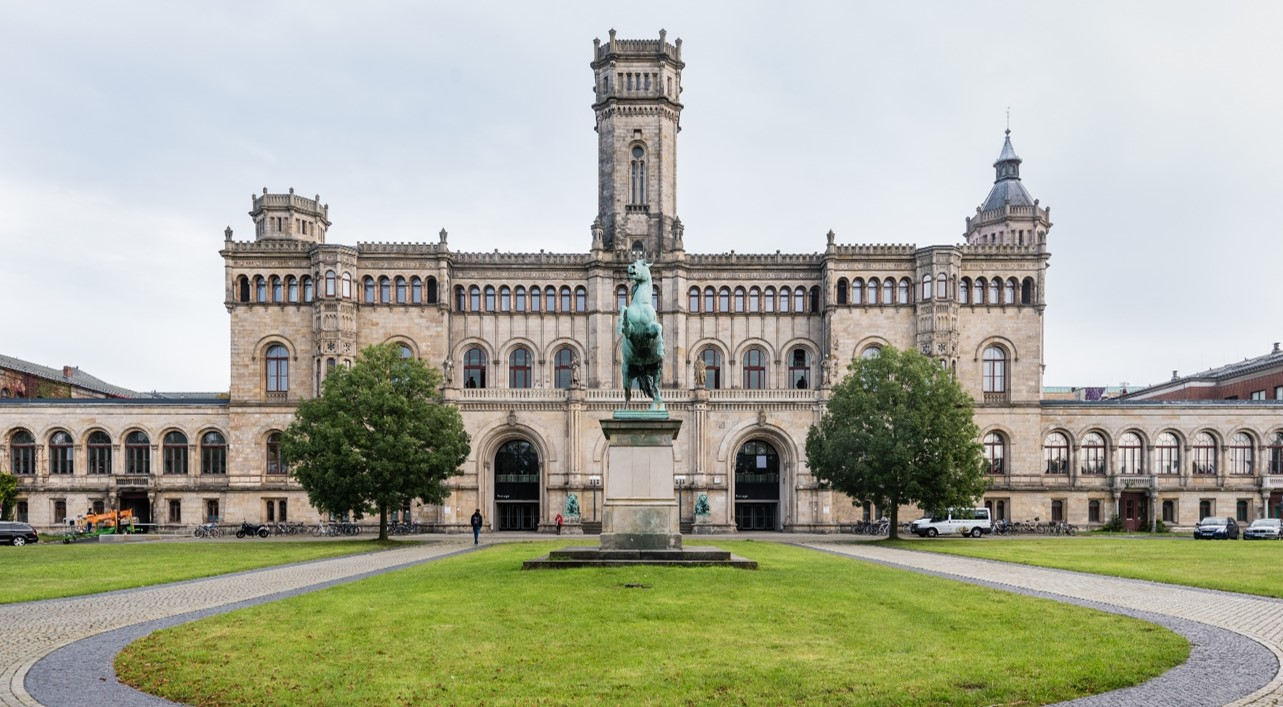
\includegraphics[width=0.65\textwidth]{figures/luh_default_presentation_title_image.jpg}}

% Title page: luhstyle
% \setbeamertemplate{title page}[luhstyle]
% % Add optional title image here
% \addtitlepageimage{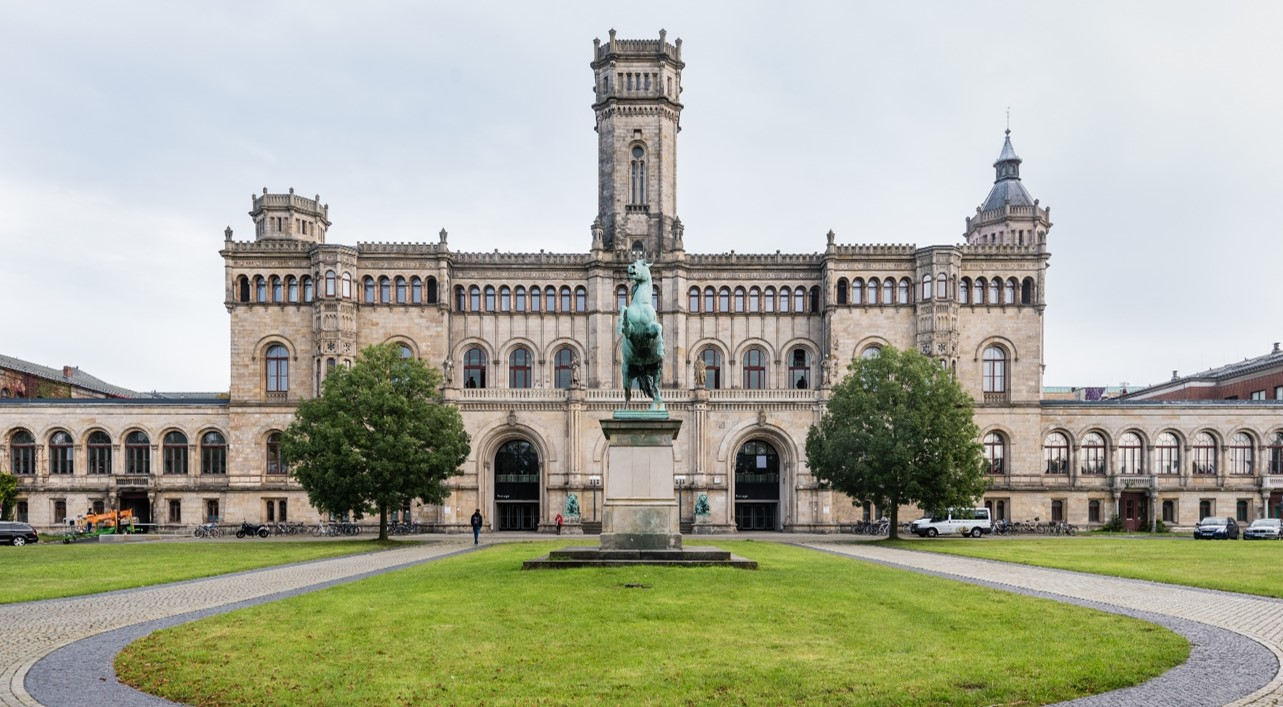
\includegraphics[width=0.75\textwidth]{figures/luh_default_presentation_title_image.jpg}}

\author[Marius Lindauer]{Marius Lindauer\\[1em]
	
\includegraphics[height=\logoheight]{../latex_main/figures/luh_logo_rgb_0_80_155.pdf}\qquad

\includegraphics[height=2.2em]{../latex_main/figures/logo_short}\qquad
%
\includegraphics[height=2.2em]{../latex_main/figures/L3S.jpg}\qquad

\includegraphics[height=2.2em]{../latex_main/figures/LAA.png}}
\date{%Winter Term 2021/22
}


%%% Custom Packages
%----------------------------------------------------------------------
% Create dummy content
\usepackage{blindtext}

% Adds a frame with the current page layout. Just call \layout inside of a frame.
\usepackage{layout}

\title[Meta-RL]{Wrap Up}
\subtitle{---}


\begin{document}
	
	\maketitle

%-----------------------------------------------------------------------
%----------------------------------------------------------------------
\begin{frame}[c]{Course Overview}
	
	\begin{enumerate}
		\item Big Picture
		\item MDP, Policy, Value Iteration
		\item Policy Evaluation
		\item Model Free Control
		\item Linear Function Approximation
		\item Deep RL
		\item Policy Gradient
		\item Exploration
		\item Meta-RL
		\item Reproducibility in RL
		\item Auto-RL
		\item Project
	\end{enumerate}
	
	\pause
	$\leadsto$ More an introduction into RL!
	
\end{frame}
%----------------------------------------------------------------------
%----------------------------------------------------------------------
\begin{frame}[c]{Further and Related Topics}
	
	\begin{itemize}
	    \item Model-based RL
	    \item Multi-Agent RL
	    \item Imitation Learning
	    \item Transfer Learning
	    \item Offline (Batch) RL
	    \item Control + Planning (e.g., MCTS)
	    \item Game Theory
	    \item \ldots
	\end{itemize}
\end{frame}
%----------------------------------------------------------------------
%----------------------------------------------------------------------
\begin{frame}[c]{AI Lectures at LUH}
	
	\centering
	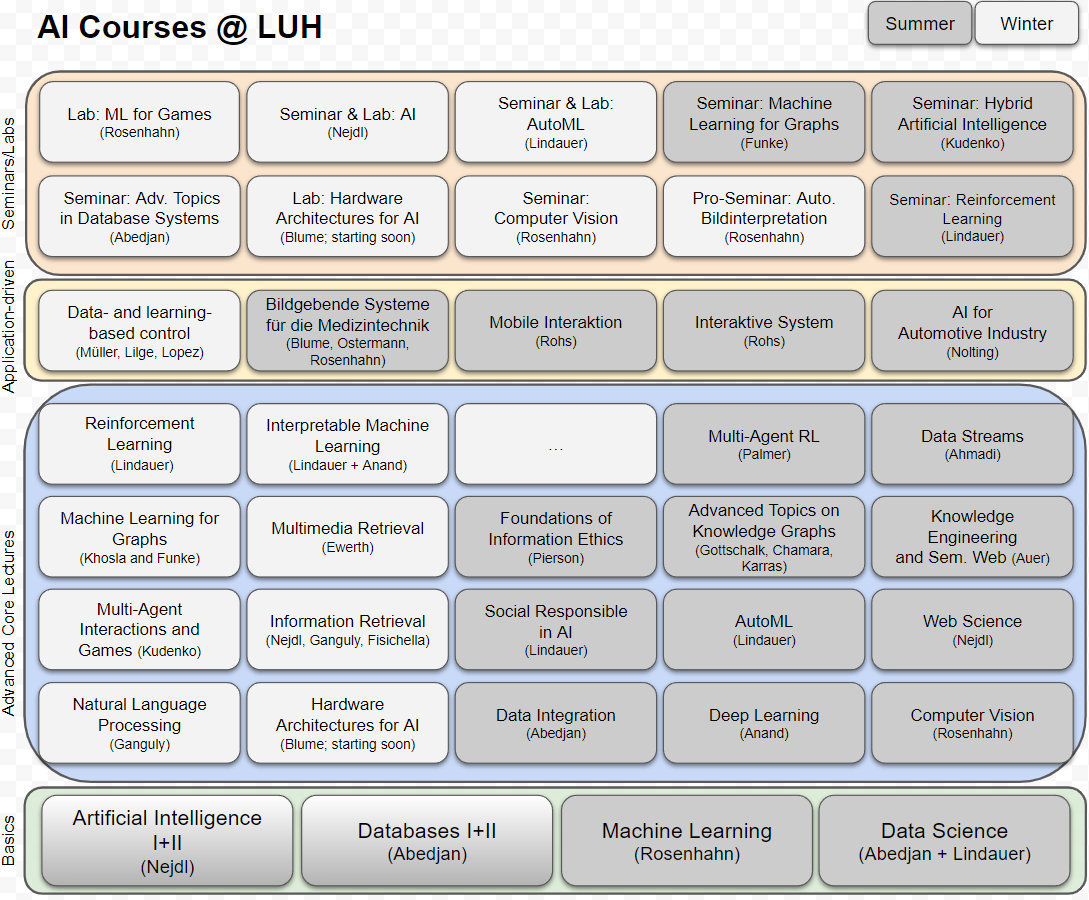
\includegraphics[width=0.54\textwidth]{w11_wrap_up/images/ai_courses_luh.PNG}
	
\end{frame}
%----------------------------------------------------------------------
%----------------------------------------------------------------------
\begin{frame}[c]{}
	
	\centering
	\huge
	Overview on Possible Master Thesis Topics with Us
	
\end{frame}
%----------------------------------------------------------------------
%----------------------------------------------------------------------
\begin{frame}[c]{Multi-Fidelity Evaluations for cRL}
	
    \begin{itemize}
		\item Level: MSc Thesis
		\item Idea in a nutshell:
		\begin{itemize}
		    \item Evaluating contextual RL is expensive, but important for assessing the true performance
		    \item Multi-fidelity allows us to use partial information (e.g., evaluation on less instances, less steps or shorter episodes)
		    \item What does the correlation of evaluation method and true performance tell us about our algorithms?
		    \item Evaluation on CARL (Context Adaptive Reinforcement Learning benchmark library)
		\end{itemize}
		\item Requirements: Python, Hands-on RL
		\item Supervisor: Theresa Eimer / Carolin Benjamins
	\end{itemize}
	
\end{frame}
%----------------------------------------------------------------------
%----------------------------------------------------------------------
\begin{frame}[c]{Bootstrapped Meta-Learning in cRL}
	
    \begin{itemize}
		\item Level: MSc Thesis
		\item Idea in a nutshell:
		\begin{itemize}
		    \item Efficient and generalizable meta-learning is hard to achieve
		    \item Bootstrap meta-learning bootstraps a task from a meta-learner and minimizes the distance to that task under some meta-metric
		    \item Can we generalize this idea to contextual RL?
		    \item What is the relationship between the RL and generalization meta-loss landscape?
		    \item Evaluation on CARL (Context Adaptive Reinforcement Learning benchmark library)
		\end{itemize}
		\item Requirements: Python, Hands-on DL, AutoML
		\item Supervisor: Theresa Eimer
	\end{itemize}
	
\end{frame}
%----------------------------------------------------------------------
% %----------------------------------------------------------------------
% \begin{frame}[c]{FACT optimization in the Outer Loop}
	
% \begin{itemize}
%     \begin{itemize}
% 		\item Level: MSc Thesis
% 		\item Idea in a nutshell:
% 		\begin{itemize}
% 		    \item FACT = fairness, accountability, transparency 
% 		    \item How can we make use of (multi-objective) AutoML for FACT optimization?
% 		    \item Comparison to inner loop optimization, impact of different design decisions, use of multi-fidelity methods
% 		\end{itemize}
% 		\item Requirements: Python, AutoML, Hands-On ML (/RL)
% 		\item Supervisor: Theresa Eimer
% 	\end{itemize}
% \end{itemize}
	
% \end{frame}
% %----------------------------------------------------------------------
%----------------------------------------------------------------------
\begin{frame}[c]{Metrics of Generalization in CARL}
	
    \begin{itemize}
		\item Level: MSc Thesis
		\item Idea in a nutshell:
		\begin{itemize}
		    \item CARL: Context Adaptive Reinforcement Learning benchmark library
		    \item We as humans do not need an explicit context information to learn how to generalize between tasks (e.g., we can easily grab different kinds of bottles without thinking about shape, size and weight of it)
		    \item How can we learn/estimate what is useful context information for generalization?
		    \item What is a good metric to compare the information degree of context information without expensive training of agents?
		    \item Evaluation on CARL (Context Adaptive Reinforcement Learning benchmark library)
		\end{itemize}
		\item Requirements: Python, Hands-on RL
		\item Supervisor: Aditya Mohan
	\end{itemize}
	
\end{frame}
%----------------------------------------------------------------------
%----------------------------------------------------------------------
\begin{frame}[c]{Context-Agnostic Latent Representations}
	
    \begin{itemize}
		\item Level: MSc Thesis
		\item Idea in a nutshell:
		\begin{itemize}
		    \item Besides explicit context information, we can observe what kind of states the agent observes, how the transitions work and what kind of reward signal it gets
		    \item Can we make use of it to learn an latent embedding over the training tasks?
		    \item Test it on the test tasks in a zero-short policy transfer scenario?
		    \item Study and visualize the context space and check information degree compared to explicit context information
		    \item Evaluation on CARL (Context Adaptive Reinforcement Learning benchmark library)
		\end{itemize}
		\item Requirements: Python, Hands-on RL
		\item Supervisor: Aditya Mohan
	\end{itemize}
	
\end{frame}
%----------------------------------------------------------------------
%----------------------------------------------------------------------
\begin{frame}[c]{Model-based RL for cRL}
	
    \begin{itemize}
		\item Level: MSc Thesis
		\item Idea in a nutshell:
		\begin{itemize}
		    \item Model-based RL aims at learning the MDP (i.e,, tranisition dynamics and reward signal)
		    \item for contextual RL with many MDPs, this gets much more complicated
		    \item How can we efficiently extend model-based RL to contextual RL  with joint models?
		    \item Evaluation on CARL (Context Adaptive Reinforcement Learning benchmark library)
		\end{itemize}
		\item Requirements: Python, Hands-on RL
		\item Supervisor: Carolin Benjamins
	\end{itemize}
	
\end{frame}
%----------------------------------------------------------------------
%----------------------------------------------------------------------
\begin{frame}[c]{Context Changes during Episodes}
	
    \begin{itemize}
		\item Level: MSc Thesis
		\item Idea in a nutshell:
		\begin{itemize}
		    \item So far, we always considered stationary MDPs 
		    \item What would happen if the MDP changes over time? $\leadsto$ non-stationary MDPs 
		    \item How can we combine this idea with contextual RL? 
		    \item How should an agent handle the situation if the context and the corresponding context information changes over time?
		    \item Evaluation on CARL (Context Adaptive Reinforcement Learning benchmark library)
		\end{itemize}
		\item Requirements: Python, Hands-on RL
		\item Supervisor: Carolin Benjamins
	\end{itemize}
	
\end{frame}
%----------------------------------------------------------------------

\end{document}
